\documentclass[12pt]{report}

% Languages and fonts
\usepackage{polyglossia}
\setdefaultlanguage{greek}
\setotherlanguage{english}
\usepackage{fontspec}
\renewcommand{\thesection}{\arabic{section}} % Begin sections from 1
\setmainfont{Times New Roman} % Set main font to Times New Roman

% Images
\usepackage{graphicx}
\usepackage{float} % placement of figures

% Math
\usepackage{amsmath} % mathematica symbols 
\usepackage{mathrsfs} % curly math letters
\usepackage{amssymb} %more mathematical symbols
\usepackage{gensymb} % degree symbol
\usepackage{mathtools} % For \mathclap

% Miscellaneous
\usepackage{parskip} % Remove paragraph indentation
\usepackage{enumitem} % For custom itemizes
\usepackage{hyperref} % For hyperlinks and references
\usepackage{tcolorbox} % For colored boxes

\begin{document}

\begin{titlepage}
\begin{center}
    \begin{figure}[h]
        \centering
        
\includegraphics[width=1\textwidth]{figures/auth_logo.png}
    \end{figure}

    \vspace{1cm}

    \Huge
    \textbf{4η Εργασία}

    \vspace{2cm}
    
    Υπολογιστική Νοημοσύνη \\

    \vspace{2cm}

    \Large
    Παπαδάκης Κωνσταντίνος Φώτιος \\
    ΑΕΜ: 10371

    \vfill

    \large
    Αριστοτέλειο Πανεπιστήμιο Θεσσαλονίκης \\
    Τμήμα Ηλεκτρολόγων Μηχανικών και Μηχανικών Υπολογιστών \\
    \today
\end{center}
\end{titlepage}

\tableofcontents

\newpage

\section{Εισαγωγή}
Στην τελευταία εργασία του μαθήματος θα ασχοληθούμε με την χρήση TSK (Takagi Sugeno Kang) μοντέλων προκειμένου να ταξινομήσουμε δύο διαφορετικά Datasets. Στη πρώτη περίπτωση εξετάζουμε την διαδικασία εκπαίδευσης ενώ στη δεύτερη εμβαθύνουμε προεπεξεργάζοντας τα δεδομένα και δοκιμάζοντας μεθόδους βελτιστοποίησης του μοντέλου μας. 

\section{Απλό Dataset}
Το πρώτο ασαφές νευρωνικό δίκτυο μας θα το εκπαιδεύσουμε πάνω στο ``Haberman's Survival'' Dataset του UCI repository, το οποίο αποτελείται από 306 samples και 3 χαρακτηριστικά.

\subsection{Γραφικές Παραστάσεις}
Αρχικά θα εξετάσουμε τις συναρτήσεις συμμετοχής των χαρακτηριστικών μας. Από την μία πλευρά έχουμε τις class independent συναρτήσεις συμμετοχής δημιουργήθηκαν από την συνάρτηση \textbf{genfis()} αυτόματα.

\begin{figure}[H]
    \centering
    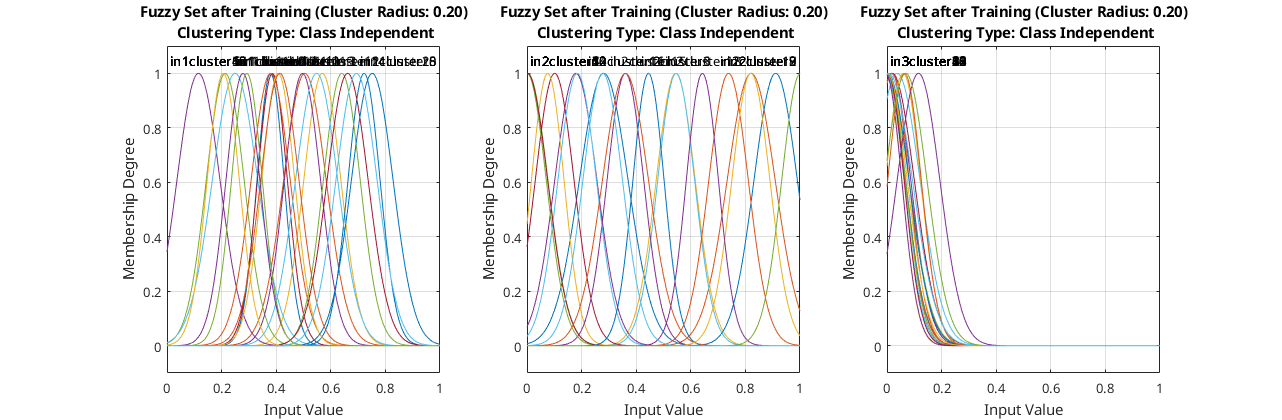
\includegraphics[width=1\textwidth]{figures/class_mf_ci_02.png}
    \label{fig:class_mf_ci_02}
\end{figure}
\begin{figure}[H]
    \centering
    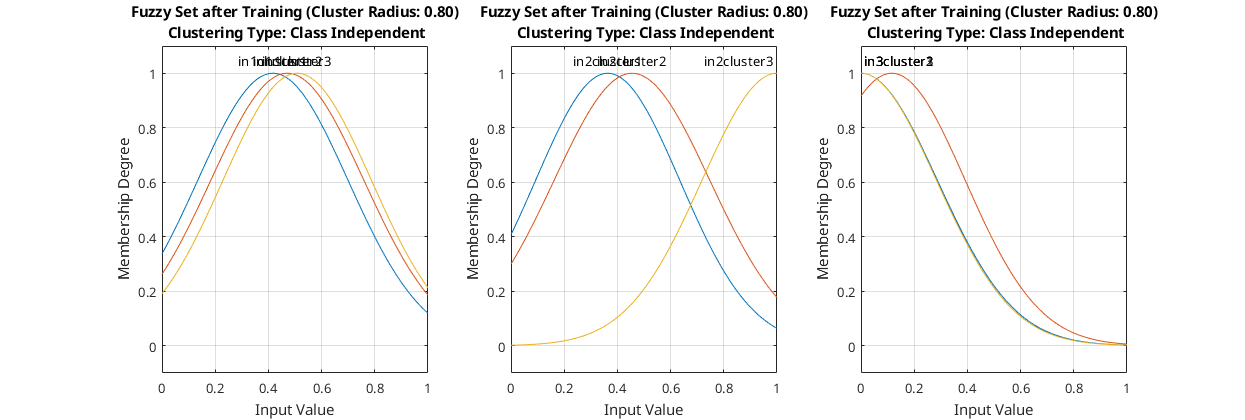
\includegraphics[width=1\textwidth]{figures/class_mf_ci_08.png}
    \label{fig:class_mf_ci_08}
\end{figure}

Από την άλλη πλευρά, έχουμε τις class dependent συναρτήσεις συμμετοχής, οι οποίες δημιουργήθηκαν χειροκίνητα μέσω των clusters που δημιουργήσαμε από τα training data κάνοντας χρήση της συνάρτησης \textbf{subclust()}.

\begin{figure}[H]
    \centering
    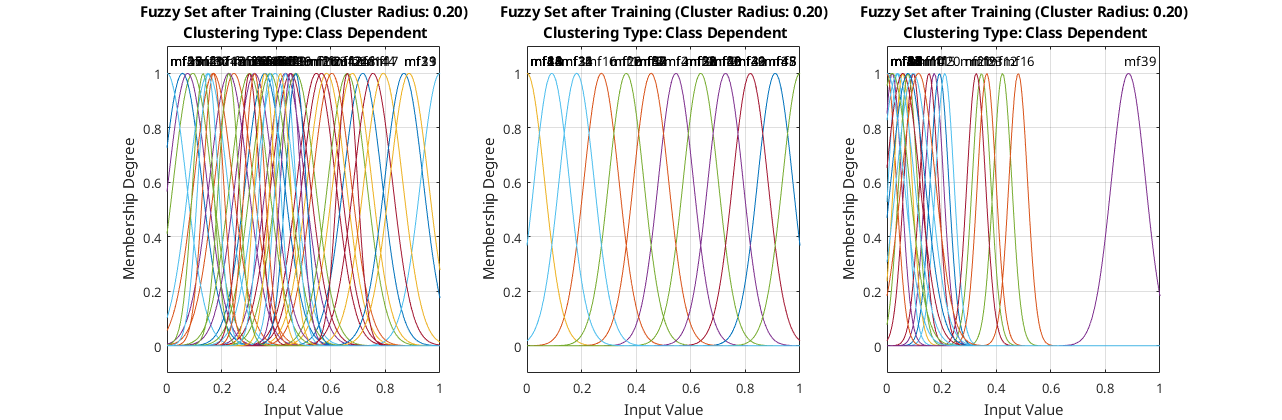
\includegraphics[width=1\textwidth]{figures/class_mf_cd_02.png}
    \label{fig:class_mf_cd_02}
\end{figure}
\begin{figure}[H]
    \centering
    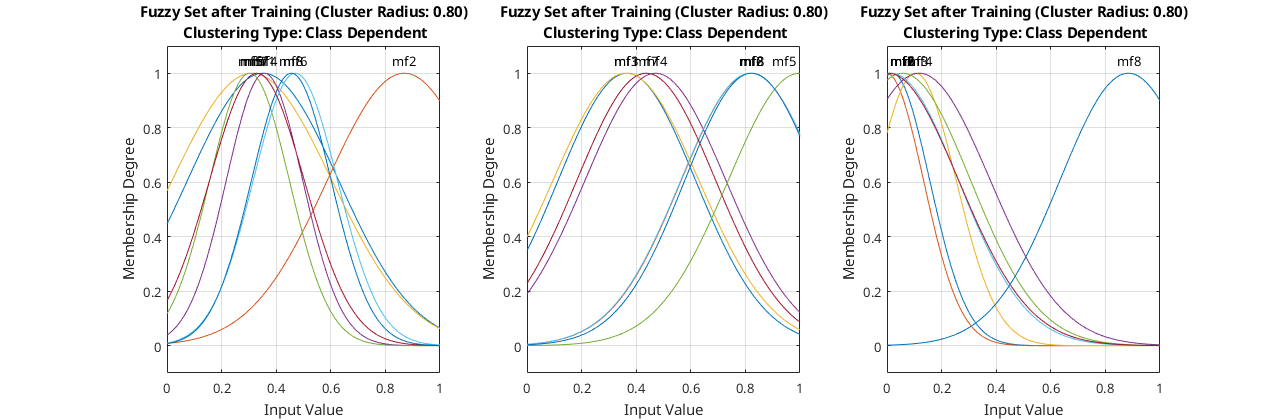
\includegraphics[width=1\textwidth]{figures/class_mf_cd_08.png}
    \label{fig:class_mf_cd_08}
\end{figure}

Η καμπύλη εκπαίδευσης των τεσσάρων μοντέλων φαίνεται παρακάτω. Το class independent μοντέλο με ακτίνα 0.2 είναι το πιο αναξιόπιστο με τους λιγότερους κανόνες. Το σφάλμα εκπαίδευσης είναι αρκετά χαμηλό, όμως το σφάλμα επικύρωσης είναι εξαιρετικά υψηλό και ασταθές. Όλα τα υπόλοιπα μοντέλα αρκετά καλή απόδοση.
\begin{figure}[H]
    \centering
    \begin{minipage}{0.48\textwidth}
        \centering
        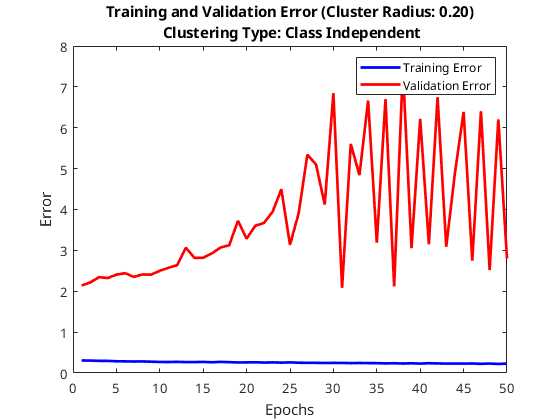
\includegraphics[width=\textwidth]{figures/class_learning_curve_ci_02.png}
        \label{fig:class_learning_curve_ci_02}
    \end{minipage}
    \hfill
    \begin{minipage}{0.48\textwidth}
        \centering
        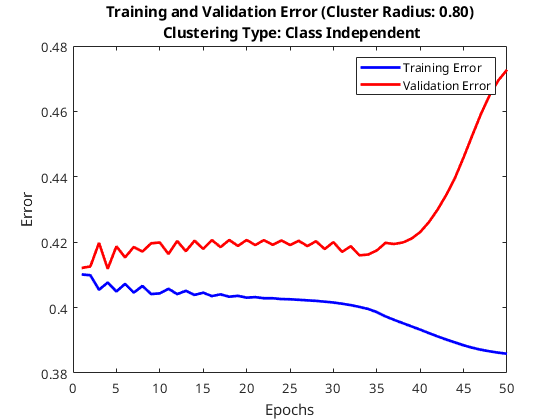
\includegraphics[width=\textwidth]{figures/class_learning_curve_ci_08.png}
        \label{fig:class_learning_curve_ci_08}
    \end{minipage}
    \caption{Class Independent Learning Curves}
\end{figure}

\begin{figure}[H]
    \centering
    \begin{minipage}{0.48\textwidth}
        \centering
        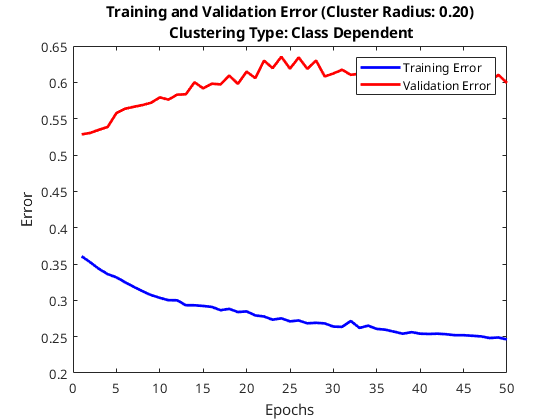
\includegraphics[width=\textwidth]{figures/class_learning_curve_cd_02.png}
        \label{fig:class_learning_curve_cd_02}
    \end{minipage}
    \hfill
    \begin{minipage}{0.48\textwidth}
        \centering
        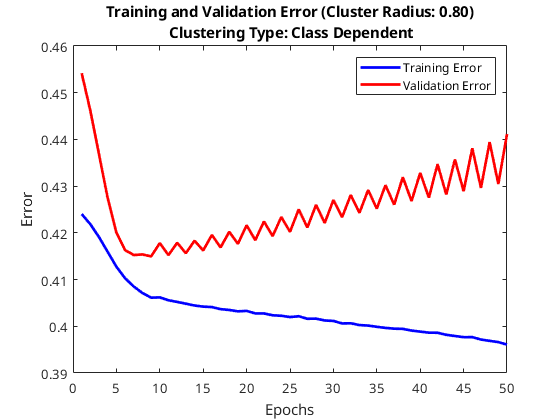
\includegraphics[width=\textwidth]{figures/class_learning_curve_cd_08.png}
        \label{fig:class_learning_curve_cd_08}
    \end{minipage}
    \caption{Class Dependent Learning Curves}
\end{figure}

Τέλος έχουμε τους πίνακες με τις ειδικές πληροφορίες κάθε μοντέλο, οι οποίοι τυπώνονται από το πρόγραμμα \textbf{classification.m} στο τέλος κάθε επανάληψης του βρόγχου που διατρέχει όλες τις ακτίνες. Για βαθύτερη ανάλυση εμπλουτίζω τη λίστα ακτινών με 0.4, 0,6 σε συνδυασμό με τις ήδη υπάρχουσες 0.2 και 0.8 μόνο στο πρόγραμμα, για να διατηρήσω συνοπτική την παρουσίαση των αποτελεσμάτων. Επίσης αύξησα τον αριθμό εποχών στις 100 για να είναι πιο εμφανή φαινόμενα όπως overfitting και underfitting.

\begin{table}[H]
    \centering
    \caption{Model 1 -- Class Independent, Radius = 0.20}
    \begin{tabular}{ll}
    \hline
    Training RMSE & 0.206935 \\
    Checking RMSE & 2.0836 \\
    Number of Rules & 20 \\
    Error Matrix & $\begin{bmatrix} 34 & 11 \\ 11 & 5 \end{bmatrix}$ \\
    Overall Accuracy (OA) & 0.6393 \\
    Producer's Accuracy (PA) & 0.7556, 0.3125 \\
    User's Accuracy (UA) & 0.7556, 0.3125 \\
    Kappa ($\hat{K}$) & 0.4117 \\
    \hline
    \end{tabular}
\end{table}

\begin{table}[H]
    \centering
    \caption{Model 2 -- Class Independent, Radius = 0.80}
    \begin{tabular}{ll}
    \hline
    Training RMSE & 0.383046 \\
    Checking RMSE & 0.411869 \\
    Number of Rules & 3 \\
    Error Matrix & $\begin{bmatrix} 41 & 15 \\ 4 & 1 \end{bmatrix}$ \\
    Overall Accuracy (OA) & 0.6885 \\
    Producer's Accuracy (PA) & 0.7321, 0.2000 \\
    User's Accuracy (UA) & 0.9111, 0.0625 \\
    Kappa ($\hat{K}$) & 0.4919 \\
    \hline
    \end{tabular}
\end{table}

\begin{table}[H]
    \centering
    \caption{Model 3 -- Class Dependent, Radius = 0.20}
    \begin{tabular}{ll}
    \hline
    Training RMSE & 0.205616 \\
    Checking RMSE & 0.528371 \\
    Number of Rules & 48 \\
    Error Matrix & $\begin{bmatrix} 42 & 14 \\ 3 & 2 \end{bmatrix}$ \\
    Overall Accuracy (OA) & 0.7213 \\
    Producer's Accuracy (PA) & 0.7500, 0.4000 \\
    User's Accuracy (UA) & 0.9333, 0.1250 \\
    Kappa ($\hat{K}$) & 0.5454 \\
    \hline
    \end{tabular}
\end{table}

\begin{table}[H]
    \centering
    \caption{Model 4 -- Class Dependent, Radius = 0.80}
    \begin{tabular}{ll}
    \hline
    Training RMSE & 0.381204 \\
    Checking RMSE & 0.414959 \\
    Number of Rules & 8 \\
    Error Matrix & $\begin{bmatrix} 44 & 12 \\ 1 & 4 \end{bmatrix}$ \\
    Overall Accuracy (OA) & 0.7869 \\
    Producer's Accuracy (PA) & 0.7857, 0.8000 \\
    User's Accuracy (UA) & 0.9778, 0.2500 \\
    Kappa ($\hat{K}$) & 0.6523 \\
    \hline
    \end{tabular}
\end{table}

\subsection{Σχολιασμός Αποτελεσμάτων}
Από τις γραφικές παραστάσεις συμπεραίνουμε ότι η μικρότερη ακτίνα δείχνει να έχει χαμηλό σφάλμα εκπαίδευσης όμως γενικεύει πολύ χειρότερα από ότι μια μεγαλύτερη. Παράλληλα διαμορφώνει πολλούς κανόνες λόγω των μικρών clusters που δημιουργούνται έτσι μπορούμε να πούμε ότι πάρα πολλοί κανόνες μπορούν να οδηγήσουν σε overfitting όπως και παρατηρούμε πιο έντονα στα μοντέλα με πολύ χαμηλή ακτίνα. Να σημειωθεί ότι και τα μοντέλα με μεγάλη ακτίνα παρουσιάζουν overfitting, όμως σε μικρότερο βαθμό και πιο σταδιακά, μετά από περισσότερες εποχές.

Επιπλέον, όταν κοιτάμε τις συναρτήσεις συμμετοχής των class dependent σε σχέση με τις class independent, παρατηρούμε ότι οι class dependent συναρτήσεις είναι πιο απλωμένες στο χώρο και ταυτόχρονα περισσότερες διότι συνδυάζουν τους μεμονωμένους κανόνες από την επιμέρους class-wise δημιουργία κανόνων.

Εν κατακλείδι, μερικές προτάσεις για βελτίωση της σχεδίασης του τμήματος υπόθεσης είναι:
\begin{itemize}
    \item Προσθήκη βαρών στους κανόνες για να δώσουμε μεγαλύτερη σημασία σε κάποιους κανόνες κατά την ταξινόμηση.
    \item Χρήση διαφορετικών μορφών συναρτήσεων συμμετοχής που μπορεί να περιγράφουν καλύτερα τα δεδομένα.
    \item Ξεχωριστό μέγεθος ακτίνας επιρροής για κάθε cluster ανάλογα με την κατανομή των δεδομένων. 
\end{itemize}


\section{Dataset υψηλής διαστασιμότητας}
Μεταβαίνοντας στο δεύτερο στάδιο της εργασίας, θα ασχοληθούμε με το ``Epileptic Seizure Recognition'' Dataset του UCI repository, το οποίο αποτελείται από 11500 samples και 178 χαρακτηριστικά, όταν αφαιρούμε τον κωδικό της πρώτης στήλης. Όπως στην τρίτη εργασία του μαθήματος, θα προεπεξεργαστούμε τα δεδομένα αυτά επιλέγοντας συγκεκριμένο αριθμό σημαντικότερων χαρακτηριστικών. Έπειτα για διαφορετικές ακτίνες tvn clusters θα επιλέξουμε τις βέλτιστες παραμέτρους μέσω k-fold cross validation και τέλος εκπαιδευσουμε το βέλτιστο μοντέλο για να το εξετάσουμε.

\subsection{Επιλογή Βέλτιστων Παραμέτρων} \label{sec:parameter_selection}
Οι πίνακας για όλες τις παραμέτρους που εξετάσαμε είναι ο εξής:
\begin{table}[H]
    \centering
    \begin{tabular}{|c|c|c|c|c|}
        \hline
        Features & Radius & AvgRMSE & AvgRules & AvgOA \\
        \hline
        5  & 0.20 & 1.1239 & 5.0    & 0.3200 \\
        5  & 0.40 & 1.1321 & 3.0    & 0.2939 \\
        5  & 0.60 & 1.2140 & 3.0    & 0.2704 \\
        5  & 0.80 & 1.4177 & 1.0    & 0.2006 \\
        10 & 0.20 & 1.0740 & 4.8    & 0.3780 \\
        10 & 0.40 & 1.0970 & 3.0    & 0.3039 \\
        10 & 0.60 & 1.2092 & 3.0    & 0.2961 \\
        10 & 0.80 & 1.4176 & 1.0    & 0.2009 \\
        15 & 0.20 & 1.0529 & 4.0    & 0.3859 \\
        15 & 0.40 & 1.0821 & 3.0    & 0.3209 \\
        15 & 0.60 & 1.1422 & 2.6    & 0.2949 \\
        15 & 0.80 & 1.4194 & 1.0    & 0.2012 \\
        20 & 0.20 & 1.0367 & 4.0    & 0.4167 \\
        20 & 0.40 & 1.0707 & 3.0    & 0.3403 \\
        20 & 0.60 & 1.1404 & 2.6    & 0.3033 \\
        20 & 0.80 & 1.4215 & 1.0    & 0.2010 \\
        \hline
    \end{tabular}
    \caption{Αποτελέσματα Επιλογής Παραμέτρων (k-fold cross validation)}
    \label{tab:parameter_selection_results}
\end{table}
\textbf{Minimum OA:} 0.4167 at Features: 20, Radius: 0.20

Παράλληλα μπορούμε να διακρίνουμε μερικά μοτίβα μέσω των παρακάτω διαγραμμάτων. Συγκεκριμένα, Το σφάλμα μειώνεται όταν πέφτει η ακτίνα των clusters, πιθανώς διότι τα δεδομένα είναι διανεμημένα σε μικρότερα clusters.

\begin{figure}[H]
    \centering
    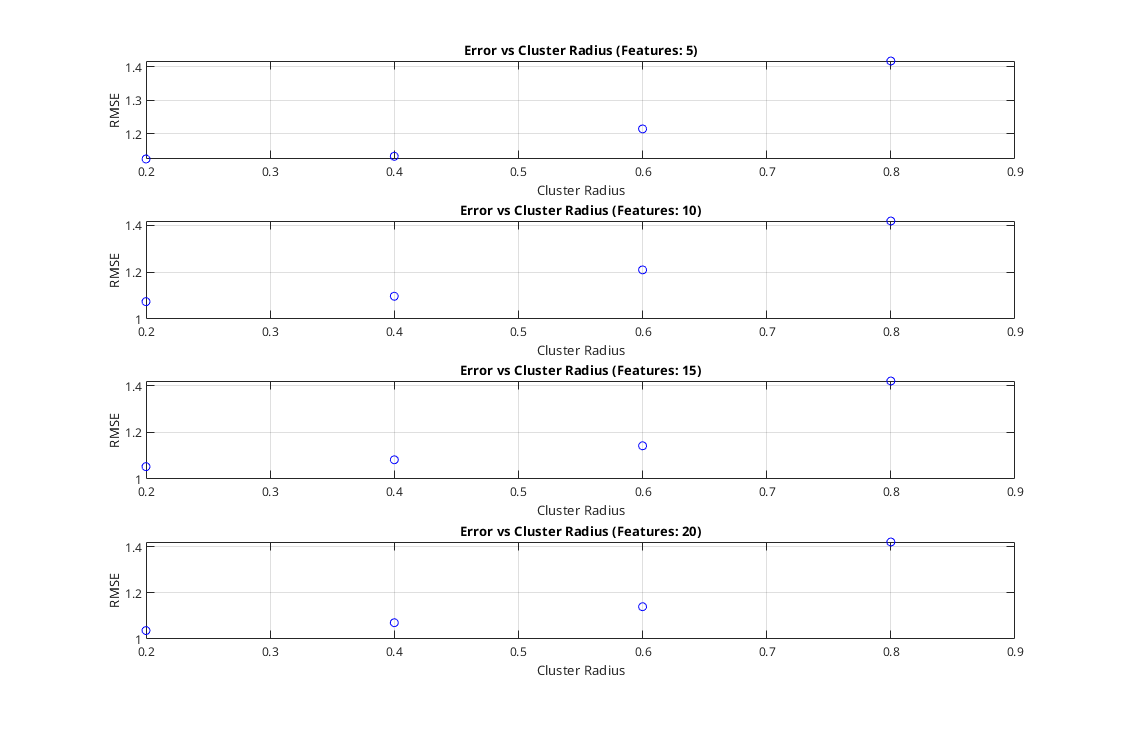
\includegraphics[width=1\textwidth]{figures/errorVScluster_radius.png}
    \caption{RMSE vs Cluster Radius}
    \label{fig:errorVScluster_radius}
\end{figure}

Επίσης, στα περισσότερα παραδείγματα αυξάνοντας τα σημαντικά χαρακτηριστικά που λαμβάνουμε υπόψιν μειώνεται το σφάλμα. Η γενική εικόνα παρουσιάζει ένα dataset το οποίο δύσκολα περιορίζεται σε λίγα χαρακτηριστικά ενώ φαίνεται να έχει αρκετά πυκνή κατανομή δεδομένων και επωφελείται από μικρότερα clusters.
\begin{figure}[H]
    \centering
    
\includegraphics[width=1\textwidth]{figures/errorVSnum_features.png}
    \caption{RMSE vs Number of Features}
    \label{fig:errorVSnum_features}
\end{figure}


\subsection{Βέλτιστο Μοντέλο} \label{sec:optimal_model}
Ενδεικτικά παραθέτουμε την μορφή των συναρτήσεων συμμετοχής πριν και μετά την εκπαίδευση του βέλτιστου μοντέλου. Παρατηρούμε πως οι συναρτήσεις συμμετοχής ταυτίζονται όταν δημιουργούνται όμως έπειτα από την εκπαίδευση του μοντέλου η κάθε μία έχει αλλάξει πλάτος και κέντρο αν και κατά κύριο λόγο μένουν όλες γύρο από κοινό κέντρο.
\begin{figure}[H]
    \centering
    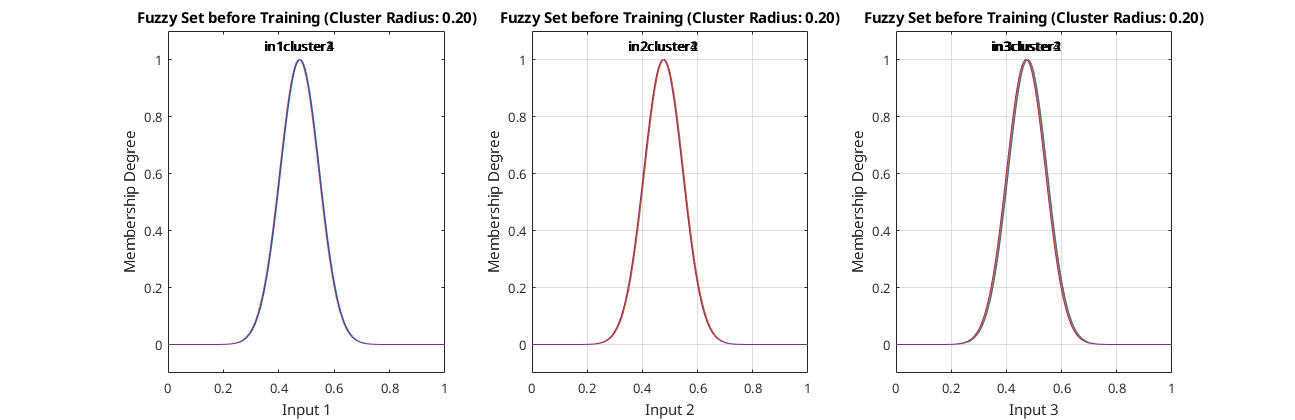
\includegraphics[width=1\textwidth]{figures/optimal_mf_before.png}
    \caption{Membership Functions Before Training}
    \label{fig:membership_functions_before_training}
\end{figure}
\begin{figure}[H]
    \centering
    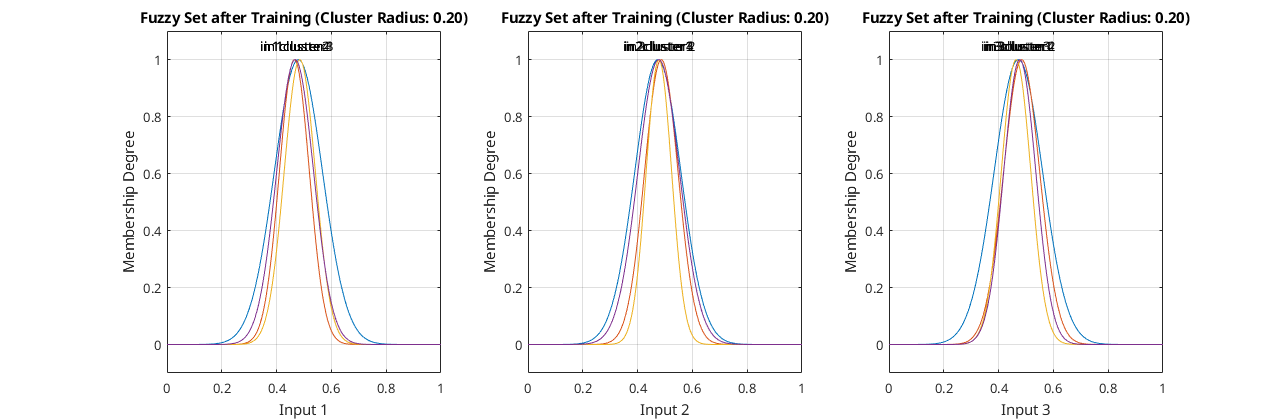
\includegraphics[width=1\textwidth]{figures/optimal_mf_after.png}
    \caption{Membership Functions After Training}
    \label{fig:membership_functions_after_training}
\end{figure}

Η καμπύλη εκπαίδευσης του βέλτιστου μοντέλου φαίνεται παρακάτω. Δεν παρατηρούμε ιδιαίτερη υπερεκπαίδευση από την στιγμή που οι καμπύλες εκπαίδευσης και επικύρωσης είναι αρκετά κοντά η μία στην άλλη.
\begin{figure}[H]
    \centering
    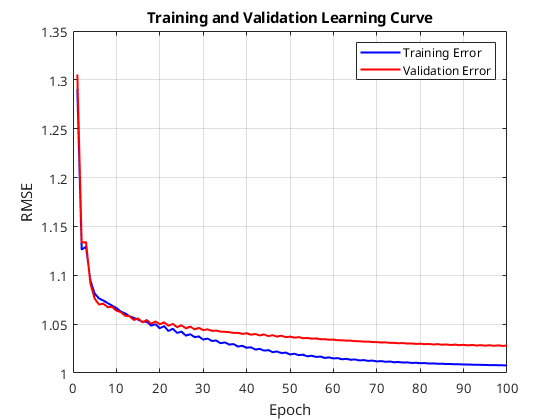
\includegraphics[width=1\textwidth]{figures/optimal_learning_curve.png}
    \caption{Learning Curve of Optimal Model}
    \label{fig:optimal_learning_curve}
\end{figure}

Επιπλέον, εδώ αποτυπώνουμε με εναν λίγο διαφορετικό τρόπο τον πίνακα σφαλμάτων, όμως πριν η έξοδος του νευρωνικού κάνει collapse σε μία συγκεκριμένη ακέραια τιμή μέσω rounding και trimming των τιμών πάνω και κάτω από τις δυνατές τιμές του label. Φαίνεται πως οι τιμές τείνουν να συγκλίνουν προς την ευθεία, η οποία συμβολίζει την ταύτιση των πραγματικών τιμών με τις προβλεπόμενες τιμές, καθώς παρατηρείται μια αυξημένη πυκνότητα σημείων προς εκείνη την διεύθυνση. 
\begin{figure}[H]
    \centering
    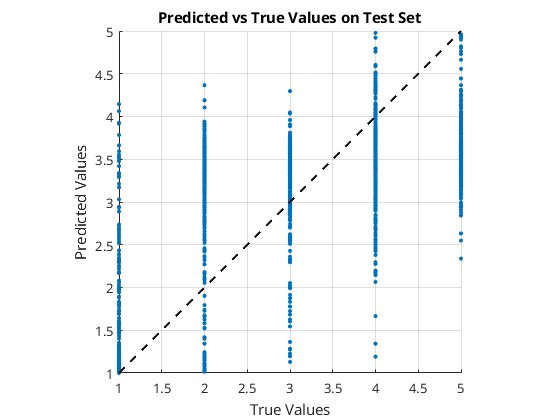
\includegraphics[width=1\textwidth]{figures/optimal_trueVSpredicted.png}
    \label{fig:optimal_trueVSpredicted}
\end{figure}

Οι πληροφορίες του βέλτιστου μοντέλου βρίσκονται παρακάτω:
\begin{tcolorbox}[title=Optimal Model, colback=gray!50, colframe=black]
Minimal training RMSE = 1.00779 \\
Minimal checking RMSE = 1.02769 \\
Cluster Radius: 0.20 \\
Number of Features: 20 \\
Number of Rules: 4 \\
Overall Accuracy (OA): 0.4113 \\
Producer's Accuracy (PA): 0.9054, 0.2250, 0.3169, 0.3235, 0.4595 \\
User's Accuracy (UA): 0.7773, 0.0570, 0.6660, 0.5431, 0.0371 \\
$\hat{K}$: 0.2642
\end{tcolorbox}

\begin{table}[H]
    \centering
    \begin{tabular}{|c|c|c|c|c|}
        \hline
        335 & 27  & 6   & 2   & 0   \\
        \hline
        57  & 27  & 19  & 16  & 1   \\
        \hline
        27  & 300 & 315 & 178 & 174 \\
        \hline
        10  & 120 & 131 & 252 & 266 \\
        \hline
        2   & 0   & 2   & 16  & 17  \\
        \hline
    \end{tabular}
    \caption{Error Matrix of Optimal Model}
\end{table}

\subsection{Σχολιασμός Αποτελεσμάτων}
Τα αποτελέσματα του βέλτιστου μοντέλου δεν είναι ιδιαίτερα θετικά με overall accuracy μόλις 0.4113. Σίγουρα είναι καλύτερο από την τυχαία ταξινόμηση (20\% accuracy). Περισσότερες πληροφορίες παραθέτονται μαζί με τα αντίστοιχα γραφήματα στα παραρτήματα \ref{sec:parameter_selection} και \ref{sec:optimal_model}.

Τέλος, όπως αναφέραμε στην προηγούμενη εργασία, στην περίπτωση που θέλαμε να προσεγγίσουμε το συγκεκριμένο πρόβλημα με grid partitioning θα είχαμε 20 χαρακτηριστικά και 2 ή 3 ασαφή σύνολα. Αυτό θα οδηγούσε σε $2^{20}$ ή $3^{20}$ κανόνες, δηλαδή 1,048,576 ή 3,486,784,401 κανόνες. Η μέθοδος subtractive clustering δημιουργεί κανόνες μόνο εκεί που αναγνωρίζει ότι υπάρχουν δεδομένα. Έτσι αποφεύγουμε την ανάγκη υπολογισμού n-διάστατων κελιών του πλέγματος η πλειονότητα των οποίων δεν θα περιέχουν δεδομένα. Εν τέλει καταλήγουμε σε 4 κανόνες, ασύγκριτα λιγότερους από ότι αν χρησιμοποιούσαμε grid partitioning.

\end{document}